\documentclass[aspectratio=169]{beamer}


\addtobeamertemplate{navigation symbols}{}{%
    \usebeamerfont{footline}%
    \usebeamercolor[fg]{footline}%
    \hspace{1em}%
    \insertframenumber/\inserttotalframenumber
}

\usepackage{booktabs, tabularx, makecell, multirow, multicol}
\newcolumntype{R}{>{\raggedleft\arraybackslash}X}
\newcolumntype{C}{>{\centering\arraybackslash}X}

\usepackage{hyperref}
\usepackage{minted}
\setminted{
    autogobble=true,
    breaklines=true,
    fontsize=\footnotesize,
}

\title{Custom Acceleration with FPGAs}
\subtitle{CS5222 -- Project 2}

\usepackage{xcolor}
\definecolor{rowhlt}{HTML}{B7D7D7}

\author{SHEN JIAMIN}
\institute{A0209166A \\ \href{mailto:shen_jiamin@u.nus.edu}{\nolinkurl{shen_jiamin@u.nus.edu}}}
\date{Mar 31, 2022}



\begin{document}

\frame{\titlepage}

\AtBeginSection[]
{
    \begin{frame}
        \frametitle{Table of Contents}
        \tableofcontents
    \end{frame}
}

\section{Experiment Environment}

\begin{frame}
    \frametitle{Experiment Environment}
    \begin{itemize}
        \item Ubuntu 20.04.4 LTS (GNU/Linux 5.4.0-105-generic x86\_64)
        \item PYNQ v2.7.0
        \item Vivado 2020.2
    \end{itemize}
\end{frame}

\begin{frame}[fragile]
    \frametitle{Problem with Vivado HLS 2017.1}

    Due to the change in glibc,
    \begin{itemize}
        \item Vivado HLS 2017.1 doesn't work on Ubuntu 20.04 or Ubuntu 18.04
        \item It can only run on Ubuntu 16.04
    \end{itemize}

    \begin{minted}[highlightlines=9,highlightcolor=rowhlt]{text}
$ vivado_hls -f hls.tcl
================================================================
  Vivado(TM) HLS - High-Level Synthesis from C, C++ and SystemC
  Version 2017.1
  Build 1846317 on Fri Apr 14 19:19:38 MDT 2017
  Copyright (C) 1986-2017 Xilinx, Inc. All Rights Reserved.
================================================================
...
/data/Xilinx/Vivado_HLS/2017.1/lnx64/tools/gcc/bin/../lib/gcc/x86_64-unknown-linux-gnu/4.6.3/include-fixed/wchar.h:175:22: fatal error: xlocale.h: No such file or directory
compilation terminated.
make: *** [csim.mk:74: obj/mmult_test.o] Error 1
ERROR: [SIM 211-100] 'csim_design' failed: compilation error(s).
    \end{minted}
\end{frame}

\begin{frame}
    \frametitle{Lift the IDE Version}

    \begin{columns}
        \column{0.4\textwidth}
        \begin{itemize}
            \item Latest release of PYNQ is v2.7.0
            \item PYNQ v2.7.0 requires Vivado 2020.2
        \end{itemize}

        \column{0.7\textwidth}
        \begin{figure}
            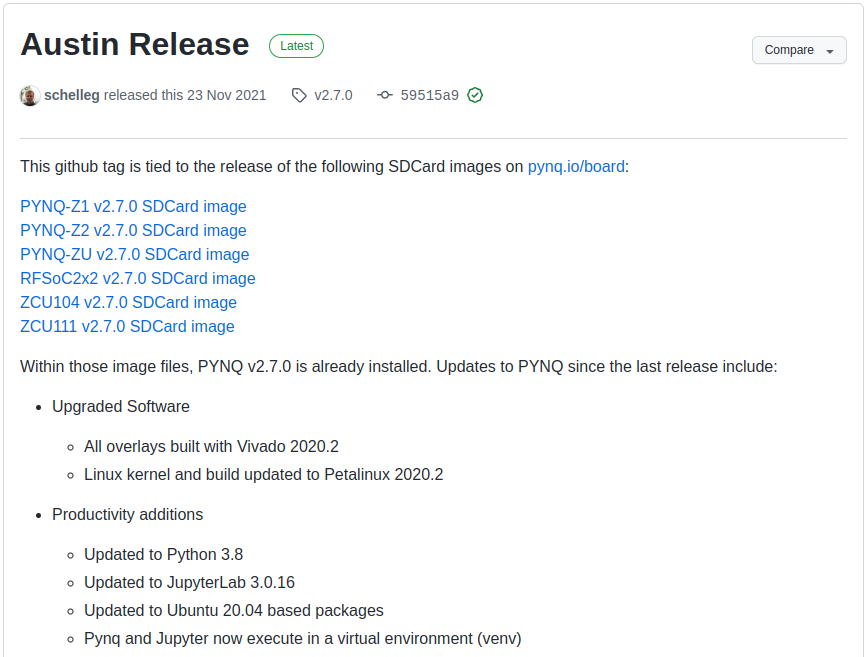
\includegraphics[scale=0.32]{images/pynq-release.png}
        \end{figure}
    \end{columns}
\end{frame}

\begin{frame}[fragile]
    \frametitle{Changes for Vivado 2020.2}
    \framesubtitle{HLS Synthesis}

    \begin{itemize}
        \item Vivado HLS is changed to Vitis HLS
              \begin{minted}{console}
            $ vitis_hls -f hls.tcl
        \end{minted}
        \item Pipelining enabled by default
              \begin{minted}{tcl}
            config_compile -pipeline_loops 0
        \end{minted}
        \item RAM can be inferred to 1WnR
              \begin{minted}{C++}
            #pragma HLS bind_storage variable=in_buf type=RAM_T2P
        \end{minted}
        \item \texttt{TLAST} signal is not generated properly.
              \begin{minted}{C++}
            void mmult_hw(hls::stream<AXI_VAL> &in_stream, hls::stream<AXI_VAL> &out_stream);
        \end{minted}
    \end{itemize}

\end{frame}


\begin{frame}[fragile]
    \frametitle{Changes for Vivado 2020.2}
    \framesubtitle{System Synthesis}

    \begin{itemize}
        \item Bypass version check in \nolinkurl{classifier.tcl}
              \begin{minted}{tcl}
            set scripts_vivado_version 2020.2
        \end{minted}
        \item Bad lexical cast: source type value could not be interpreted as target
              \begin{minted}{console}
            $ faketime -f "-1y" make
        \end{minted}
        \item Fail to export \nolinkurl{classifier.bit} and \nolinkurl{classifier.hdf}

              It doesn't matter, see next page
    \end{itemize}

\end{frame}


\begin{frame}[fragile]
    \frametitle{Changes for PYNQ v2.7.0}

    \begin{itemize}
        \item Tcl parsing removed - please generate and use an HWH file for Overlays
              \begin{minted}{console}
            $ scp `find -name "*.bit"` xilinx@ip-address:~/classifier.bit
            $ scp `find -name "*.hwh"` xilinx@ip-address:~/classifier.hwh
        \end{minted}
        \item The DMA interface has changed.
              \begin{minted}{python}
            ol = Overlay("/home/xilinx/classifier.bit")
            ol.download()

            dma_mm2s = ol.axi_dma_0
            dma_s2mm = ol.axi_dma_1
        \end{minted}
        \item DMA buffer is be typed
              \begin{minted}{python}
            output_buffer = allocate(shape=(BATCH * CLASSES,), dtype=np.float32)
            c = np.reshape(np.array(output_buffer), (BATCH, CLASSES))
        \end{minted}
    \end{itemize}

\end{frame}

\section{Result for Part 1 and Part 2}

\begin{frame}[fragile]
    \frametitle{Result for Part 1}

    \begin{table}
        \begin{tabularx}{\textwidth}{clRrl}
            \toprule
            \multicolumn{2}{c}{\multirow{2}{*}{Profile}} &
            \multicolumn{3}{c}{Latency}                                                                                                \\
            \cmidrule(lr){3-5}
                                                         &                                                 &
            \multicolumn{1}{c}{Overall}                  &
            \multicolumn{2}{c}{Normalized}                                                                                             \\
            \midrule
            A                                            & Baseline (NoPipe)                               & 228022 & 28502.8 & 1.0x   \\
            B                                            & L2 Pipelining (T2P)                             & 13885  & 1735.6  & 16.4x  \\
            C                                            & Partition (\texttt{dim}=2, \texttt{factor}=16)  & 4279   & 534.9   & 53.3x  \\
            D                                            & Amortizing (\texttt{batch}=256)                 & 57103  & 223.1   & 127.8x \\
            E                                            & Tiling (\texttt{batch}=2048, \texttt{tile}=128) & 458106 & 223.7   & 127.4x \\
            F                                            & Hardware                                        & 949242 & 463.5   & 61.5x  \\
            \bottomrule
        \end{tabularx}
    \end{table}

    On Hardare: Accuracy = 86.96\%, FPGA Speedup = 4.83x

\end{frame}

\begin{frame}
    \frametitle{Result for Part 2}
    \framesubtitle{Pre-experiment}

    \begin{figure}
        \centering
        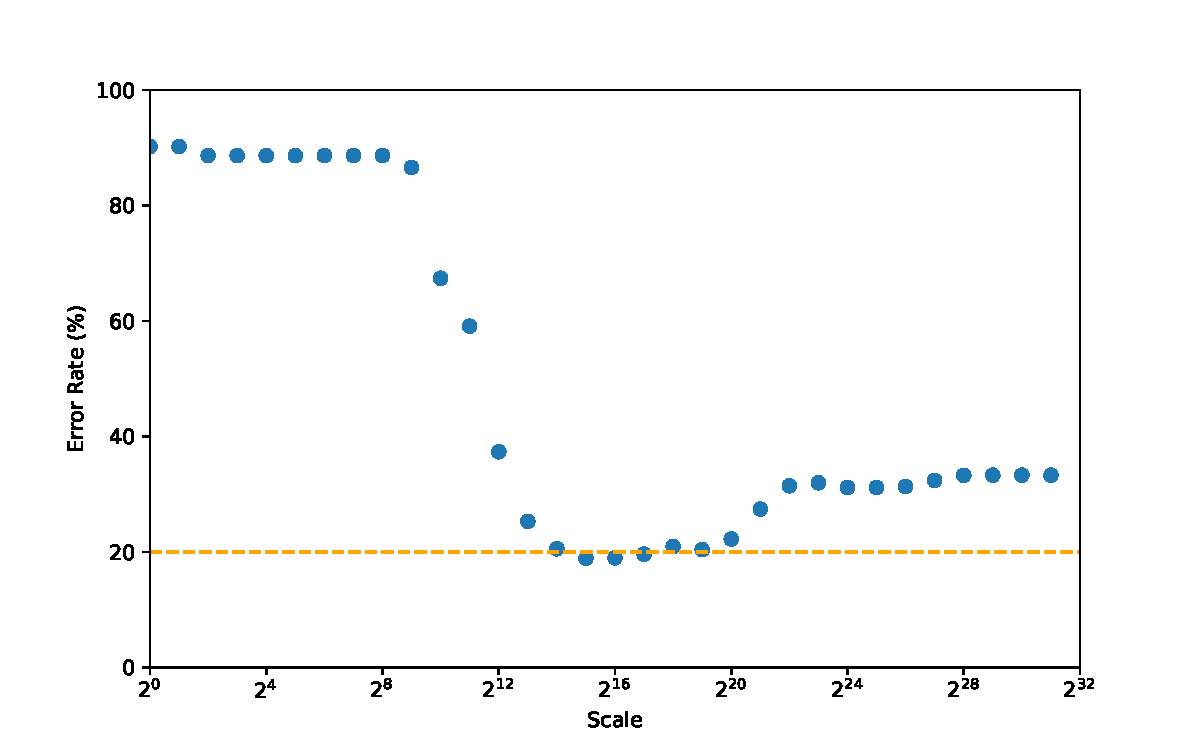
\includegraphics[scale=0.48]{images/scale_pretest.pdf}
    \end{figure}

\end{frame}

\begin{frame}
    \frametitle{Result for Part 2}
    \framesubtitle{Experiment Result}

    \begin{itemize}
        \item SCALE = \(2^{16}\)
        \item Hardware Design
              \begin{itemize}
                  \item 127 multipliers on LUT, 129 multiply-accumulate operators on DSP
                  \item Overall Latency: 386378 cycles
                  \item Normalized Latency: 467.17 cycles (604.3x)
              \end{itemize}
        \item Evaluation
              \begin{itemize}
                  \item Accuracy: 80.04\%
                  \item FPGA Speedup: 34.94x
              \end{itemize}
    \end{itemize}
\end{frame}

\section{Design for Part 3}

\begin{frame}
    \frametitle{Optimization against Latency}
    \framesubtitle{Enhancing a Single AXI Transfer}

    Expanding \texttt{TDATA} width improves the rate of transfer.
    \begin{itemize}
        \item Original design transfers 64 bits per cycle
              \begin{itemize}
                  \item A tile of 128 inputs has \(128 \times 16^2 \times 8 = 2^{18}\) bits
                  \item It needs \(2^{12} = 4096\) cycles to transfer
              \end{itemize}
        \item Expand the AXI \texttt{TDATA} bus to 256 bits
    \end{itemize}

    \begin{table}[ht!]
        \centering
        \begin{tabular}{cccc}
            \toprule
            \texttt{TDATA} width (bits) & Latency (cycles) & Trip Count \\
            \midrule
            64                          & 4096             & 128        \\
            128                         & 2048             & 128        \\
            256                         & 1024             & 128        \\
            \bottomrule
        \end{tabular}
    \end{table}

\end{frame}

\begin{frame}
    \frametitle{Optimization against Latency}
    \framesubtitle{Reducing the Input Dimension}

    Reducing input dimension lowers the number of bits to transfer (and also simplifies the computation).
    \begin{itemize}
        \item Input dimension reduced to \(8 \times 8\)
        \item Input depth reduced to 4 bits
    \end{itemize}
    But that makes the prediction accuracy declined to 82.96\%.

\end{frame}

\begin{frame}
    \frametitle{Optimization against Accuracy}

    New classifier architecture:
    \begin{itemize}
        \item Input layer: \(64 \times 16\) 8-bit integers
        \item Activation layer: ReLU
        \item Output layer: \(16 \times 10\) 8-bit integers with a bias of \(10\) 16-bit integers.
    \end{itemize}

    Prediction accuracy:
    \begin{itemize}
        \item Floating-point numbers:  89.88\%
        \item Fixed-point numbers: 88.92\%
    \end{itemize}

\end{frame}


\begin{frame}
    \frametitle{IP Synthesis}
    \framesubtitle{Latency Estimates}

    Overall Latency: 159646 cycles
    \begin{table}
        \begin{tabularx}{\textwidth}{lRRRR}
            \toprule
            \multicolumn{1}{c}{Loop}    & Latency & Iter Latency & Trip Count & Pipelined \\
            \midrule
            \texttt{- LOAD\_OFFSET}     & 10      & 1            & 10         & yes       \\
            \texttt{- LOAD\_WEIGHT1}    & 32      & 2            & 16         & yes       \\
            \texttt{- LOAD\_WEIGHT2}    & 40      & 9            & 5          & yes       \\
            \texttt{- LT}               & 159552  & 2493         & 64         & no        \\
            \texttt{ + LOAD\_INPUT}     & 128     & 1            & 128        & yes       \\
            \texttt{ + COMPUTE\_INPUT}  & 2053    & 7            & 2048       & yes       \\
            \texttt{ + COMPUTE\_OUTPUT} & 134     & 8            & 128        & yes       \\
            \texttt{ + STORE\_OUTPUT}   & 129     & 3            & 128        & yes       \\
            \bottomrule
        \end{tabularx}
    \end{table}

\end{frame}


\begin{frame}
    \frametitle{IP Synthesis}
    \framesubtitle{Utilization Estimates}

    \begin{table}
        \begin{tabular}{clc}
            \toprule
            Implementation & \multicolumn{1}{c}{Module}                    & Count \\
            \midrule
            LUT            & \texttt{mul\_8s\_4ns\_12\_1\_1}               & 32    \\
            DSP            & \texttt{mul\_mul\_16s\_8s\_16\_4\_1}          & 70    \\
            DSP            & \texttt{mac\_muladd\_16s\_8s\_16ns\_16\_4\_1} & 10    \\
            DSP            & \texttt{mac\_muladd\_16s\_8s\_16s\_16\_4\_1}  & 80    \\
            DSP            & \texttt{mac\_muladd\_8s\_4ns\_12s\_13\_4\_1}  & 32    \\
            \bottomrule
        \end{tabular}
    \end{table}

    \begin{table}
        \begin{tabularx}{\textwidth}{cRRRR}
            \toprule
            Name             & BRAM\_18K & DSP & FF   & LUT  \\
            \midrule
            Total            & 202       & 192 & 6620 & 9763 \\
            Utilization (\%) & 72        & 87  & 6    & 18   \\
            \bottomrule
        \end{tabularx}
    \end{table}

\end{frame}


\begin{frame}
    \frametitle{System Synthesis}

    Bus Interface property \texttt{TDATA\_NUM\_BYTES} does not match
    \begin{figure}
        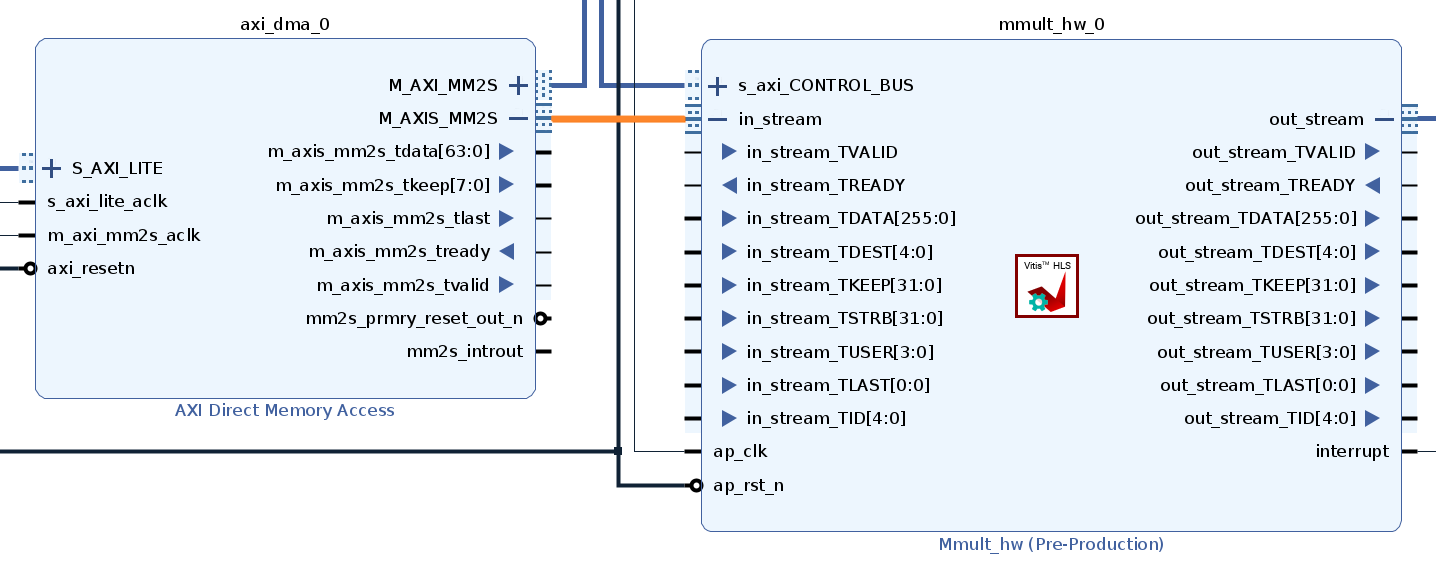
\includegraphics[scale=0.32]{images/tdata-mismatch.png}
    \end{figure}

\end{frame}

\begin{frame}
    \frametitle{Evaluation}

    \begin{itemize}
        \item Latency
              \begin{itemize}
                  \item FPGA: 3.85 ms
                  \item CPU: 169.12 ms
                  \item Speedup: 43.97x
              \end{itemize}
        \item Accuracy
              \begin{itemize}
                  \item 88.18\%
              \end{itemize}
    \end{itemize}

\end{frame}

\end{document}